\subsubsection{Exotic Higgs decays to axion-like particles: $h \to Za$ and $h \to aa$}
\begin{center}
{\it{ by Martin Bauer, Matthias Neubert, and Andrea Thamm}}
\end{center}


In this section, we discuss the exotic Higgs decays $h\to aa$ and $h\to Za$, where $a$ is a light pseudoscalar particle often called an axion-like particle (ALP). Its interactions with SM particles are described by dimension-5 operators or higher when assuming that the ALP respects a shift symmetry apart from a soft breaking through an explicit mass term \cite{Georgi:1986df} 
%
\begin{equation}\label{Leff}
\begin{aligned}
   {\cal L}_{\rm eff}^{D\le 5}
   &= \frac12 \left( \partial_\mu a\right)\!\left( \partial^\mu a\right)
    - \frac{m_{a,0}^2}{2}\,a^2 
    + \sum_f \frac{c_{ff}}{2}\,\frac{\partial^\mu a}{\Lambda}\,\bar f\gamma_\mu\gamma_5 f  + g_s^2\,C_{GG}\,\frac{a}{\Lambda}\,G_{\mu\nu}^A\,\tilde G^{\mu\nu,A} \\[-1mm]
   &\quad\mbox{}+ e^2\,C_{\gamma\gamma}\,\frac{a}{\Lambda}\,F_{\mu\nu}\,\tilde F^{\mu\nu}
    + \frac{2e^2}{s_w c_w}\,C_{\gamma Z}\,\frac{a}{\Lambda}\,F_{\mu\nu}\,\tilde Z^{\mu\nu}
    + \frac{e^2}{s_w^2 c_w^2}\,C_{ZZ}\,\frac{a}{\Lambda}\,Z_{\mu\nu}\,\tilde Z^{\mu\nu} \,,
\end{aligned}
\end{equation}
%
where $m_{a,0}$ is the explicit symmetry breaking mass term, $s_w$ and $c_w$ are the sine and cosine of the weak mixing angle, respectively, and $\Lambda$ sets the new physics scale and is related to the ALP decay constant by $\Lambda/|C_{GG}| = 32 \pi^2 f_a$. Note that an exotic $Z$-decay $Z\to\gamma a$ proceeds through the $C_{\gamma Z}$ operator.  Interactions with the Higgs boson, $\phi$, are described by the dimension-6 and 7 operators
%
\begin{equation}\label{LeffD>5}
   {\cal L}_{\rm eff}^{D\ge 6}
   = \frac{C_{ah}}{\Lambda^2} \left( \partial_\mu a\right)\!\left( \partial^\mu a\right) \phi^\dagger\phi
    + \frac{C_{Zh}}{\Lambda^3} \left( \partial^\mu a\right) 
    \left( \phi^\dagger\,iD_\mu\,\phi + \mbox{h.c.} \right) \phi^\dagger\phi + \dots  \,,
\end{equation}
%
where the first operator mediates the decay $h\to aa$, while the second one is responsible for $h\to Za$. Note that a possible dimension-5 operator coupling the ALP to the Higgs current is redundant unless it is introduced by integrating out a heavy new particle which acquires most of its mass through electroweak symmetry breaking \cite{Bauer:2016ydr,Bauer:2016zfj,Bauer:2017nlg,Bauer:2017ris}. The exotic Higgs decay rates into ALPs are given by  
 %
\begin{align}
\Gamma(h \to Za)&=\frac{m_h^3}{16\pi\,\Lambda^2}|C_{Zh}^\text{eff}|^2\lambda^{3/2}\Big(\frac{m_Z^2}{m_h^2},\frac{m_a^2}{m_h^2}\Big)\,,\\
\Gamma(h \to aa)&=\frac{m_h^3\,v^2}{32\pi\,\Lambda^4}|C_{ah}^{\rm eff}|^2\left(1-\frac{2m_a^2}{m_h^2}\right)^2\sqrt{1-\frac{4m_a^2}{m_h^2}}\,,
\end{align}
%
where $\lambda(x,y)=(1-x-y)^2-4xy$ and we define $C_{Zh}^{\rm eff} = C_{Zh}^{(5)} + C_{Zh} v^2/2 \Lambda^2$ to take into account possible contributions from a dimension-5 operator which originates from integrating out chiral heavy new physics. The relevant partial widths for this study are the decay of the ALP into photons and leptons. For the derivation and one-loop contributions we refer the reader to \cite{Bauer:2017ris}
%
\begin{align}
 \Gamma(a\to\gamma\gamma)  &= \frac{4\pi\alpha^2 m_a^3}{\Lambda^2}\,\big| C_{\gamma\gamma}^\text{eff} \big|^2 \,, \\
 \Gamma(a\to \ell^+ \ell^-)&=\frac{m_a m_\ell^2}{8\pi\Lambda^2} \left| c_{\ell\ell}^\text{eff}\right|^2 \sqrt{1-\frac{4m_\ell^2}{m_a^2}}\,.
\end{align}
%


Future hadron colliders can significantly surpass the reach of the LHC in searches for ALPs. In particular, searches for ALPs produced in exotic Higgs and $Z$ decays profit from the higher center-of-mass energies and luminosities of the proposed high-energy LHC (HE-LHC), planned to replace the LHC in the LEP tunnel with $\sqrt{s}=27 \,$TeV, and the ambitious plans for a new generation of hadron colliders with $\sqrt{s}=100\,$TeV at CERN (FCC-hh) and in China (SPPC). As benchmark scenarios we assume integrated luminosities of $3$\,ab$^{-1}$ at the LHC, $15$\,ab$^{-1}$ at the HE-LHC and $20$\,ab$^{-1}$ at the FCC-hh.
At hadron colliders, ALP production in association with electroweak bosons suffers from large backgrounds. Previous studies of these processes have therefore focussed on invisibly decaying (or stable) ALPs, taking advantage of the missing-energy signature \cite{Mimasu:2014nea,Brivio:2017ije}. In contrast, here we focus on ALPs produced in the decays of a Higgs boson, $h\to Za$ and $h \to a a$ (for more details see \cite{Bauer:2018uxu}).


%
%%% ++++++++ 
\begin{figure}
\begin{center}
 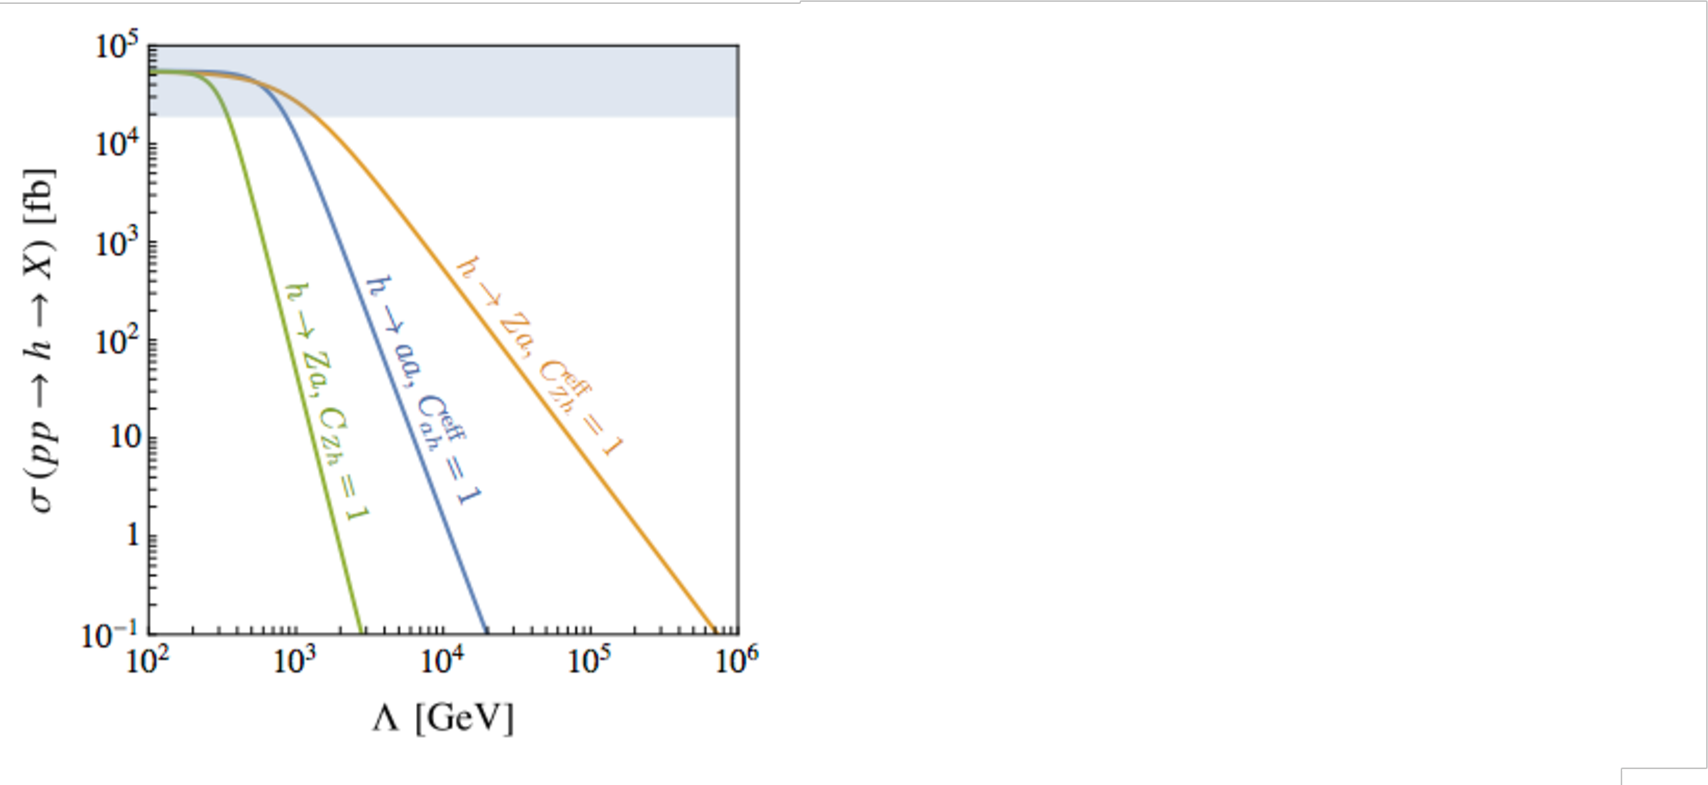
\includegraphics[width=1.3\textwidth]{\main/section9/plots/ALPs_crosssections}
    \end{center}
\caption{\label{fig:ALPpsec} Production cross sections of ALPs produced in Higgs decays at the LHC ($\sqrt{s} = 14\,$TeV) versus the new-physics scale $\Lambda$. We set $m_a=0$ and fix the relevant Wilson coefficients to 1. For the green contour we fix $C_{Zh}^{(5)}=0$ and only consider the dimension-7 coupling in \eqref{LeffD>5}.
The grey regions excluded by Higgs coupling measurements. }
%\end{center}
\end{figure}
%%% ++++++++ 
%

Exotic decays are particularly interesting, because even small couplings can lead to appreciable branching ratios and be as large as several percent \cite{Bauer:2017nlg, Bauer:2017ris}. 
This allows us to probe large new-physics scales $\Lambda$, as illustrated in Figure \ref{fig:ALPpsec}, where we show the cross sections of the processes $pp \to h \to Z a$ and $pp \to h \to aa$  at the LHC with $\sqrt{s} = 14\,$TeV. The figure nicely reflects the different scalings of the dimension-5, 6, and 7 operators in the effective ALP Lagrangian. The 
shaded region is excluded by the present Higgs coupling measurements constraining general beyond the SM decays of the Higgs boson, $\text{Br}(h\to\text{BSM})<0.34$ 
\cite{Khachatryan:2016vau}. This leads to constraints on the coefficients $|C_{Zh}^{\textrm{eff}}| < 0.72\,(\Lambda/\textrm{TeV})$ and $|C_{ah}^{\rm eff}| < 1.34\,(\Lambda/\textrm{TeV})^2$. 


%
%%% ++++++++ 
\begin{figure}[t]
\begin{center}
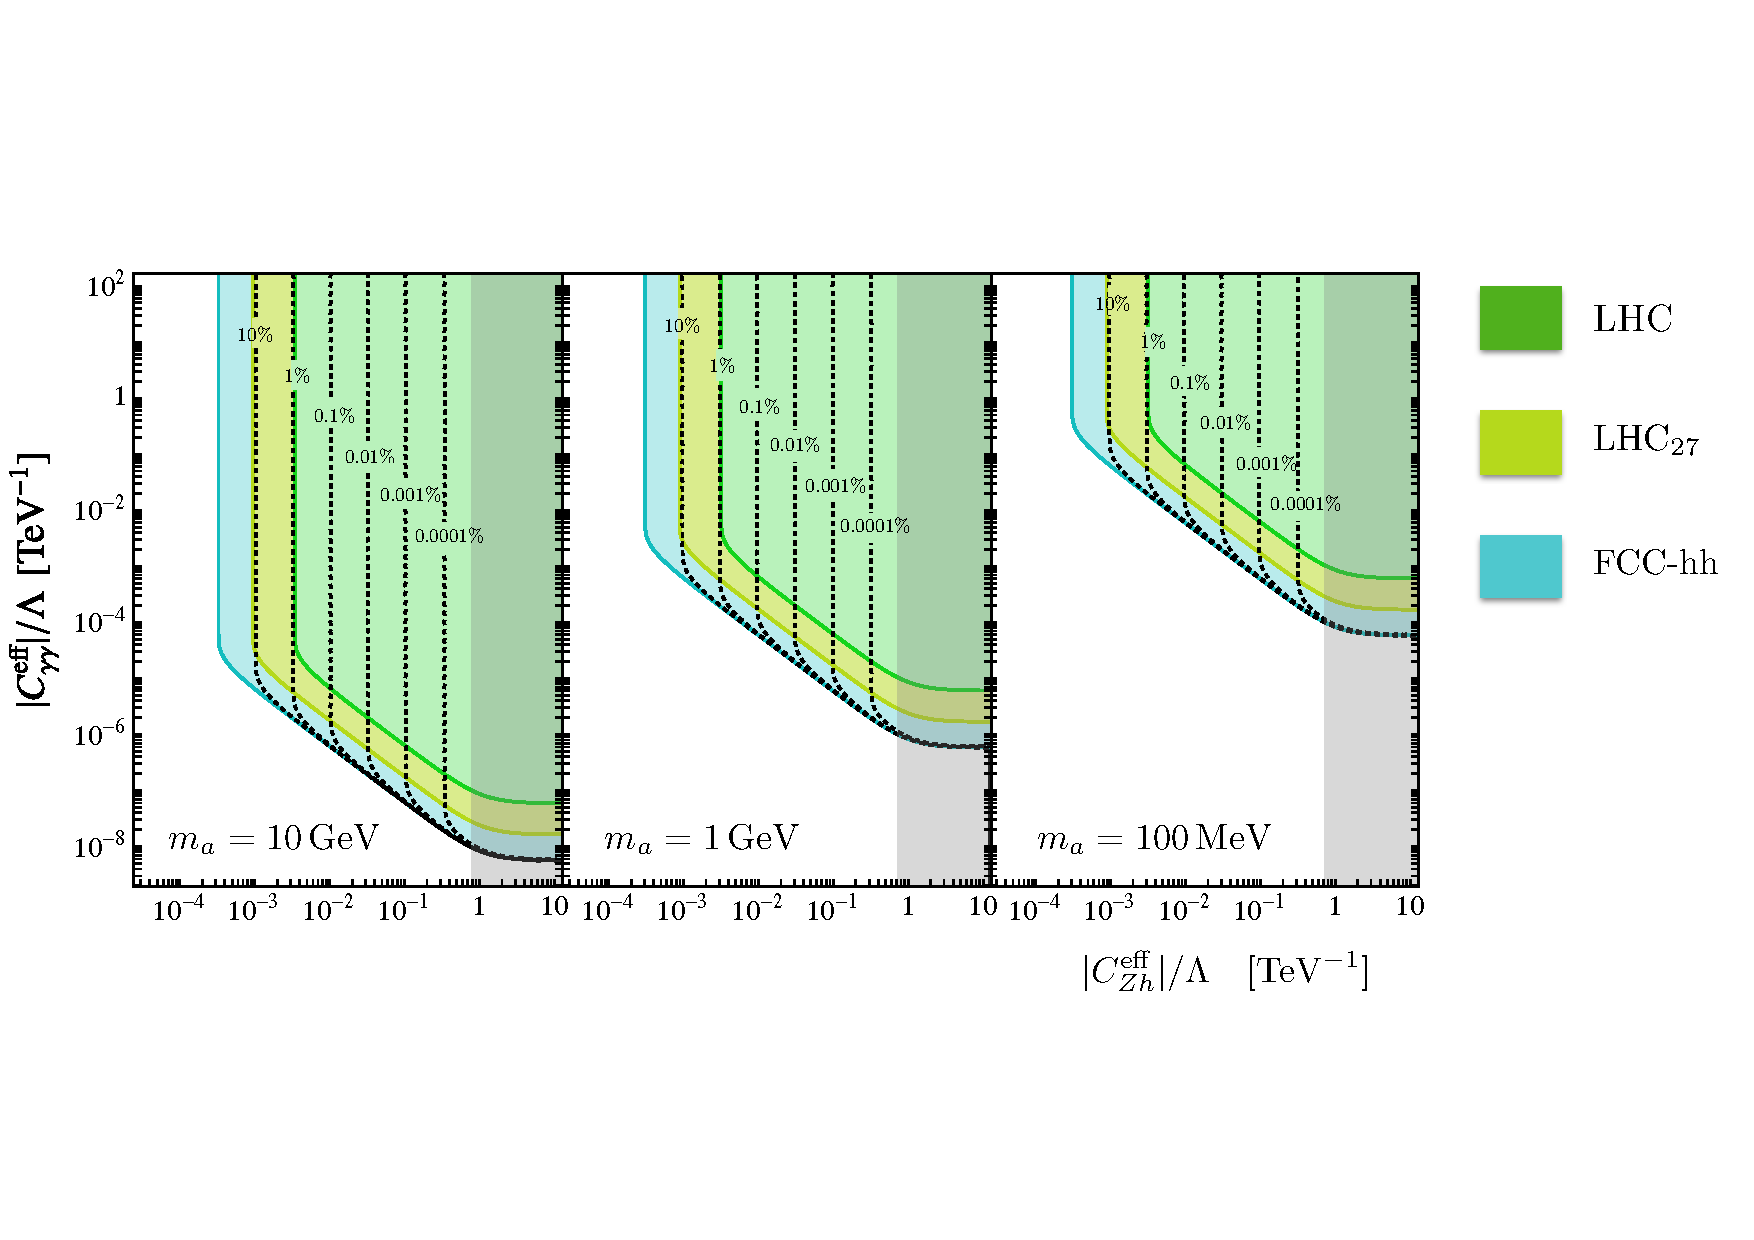
\includegraphics[width=0.85\textwidth]{\main/section9/plots/ALPs_hh_htoZa.pdf}
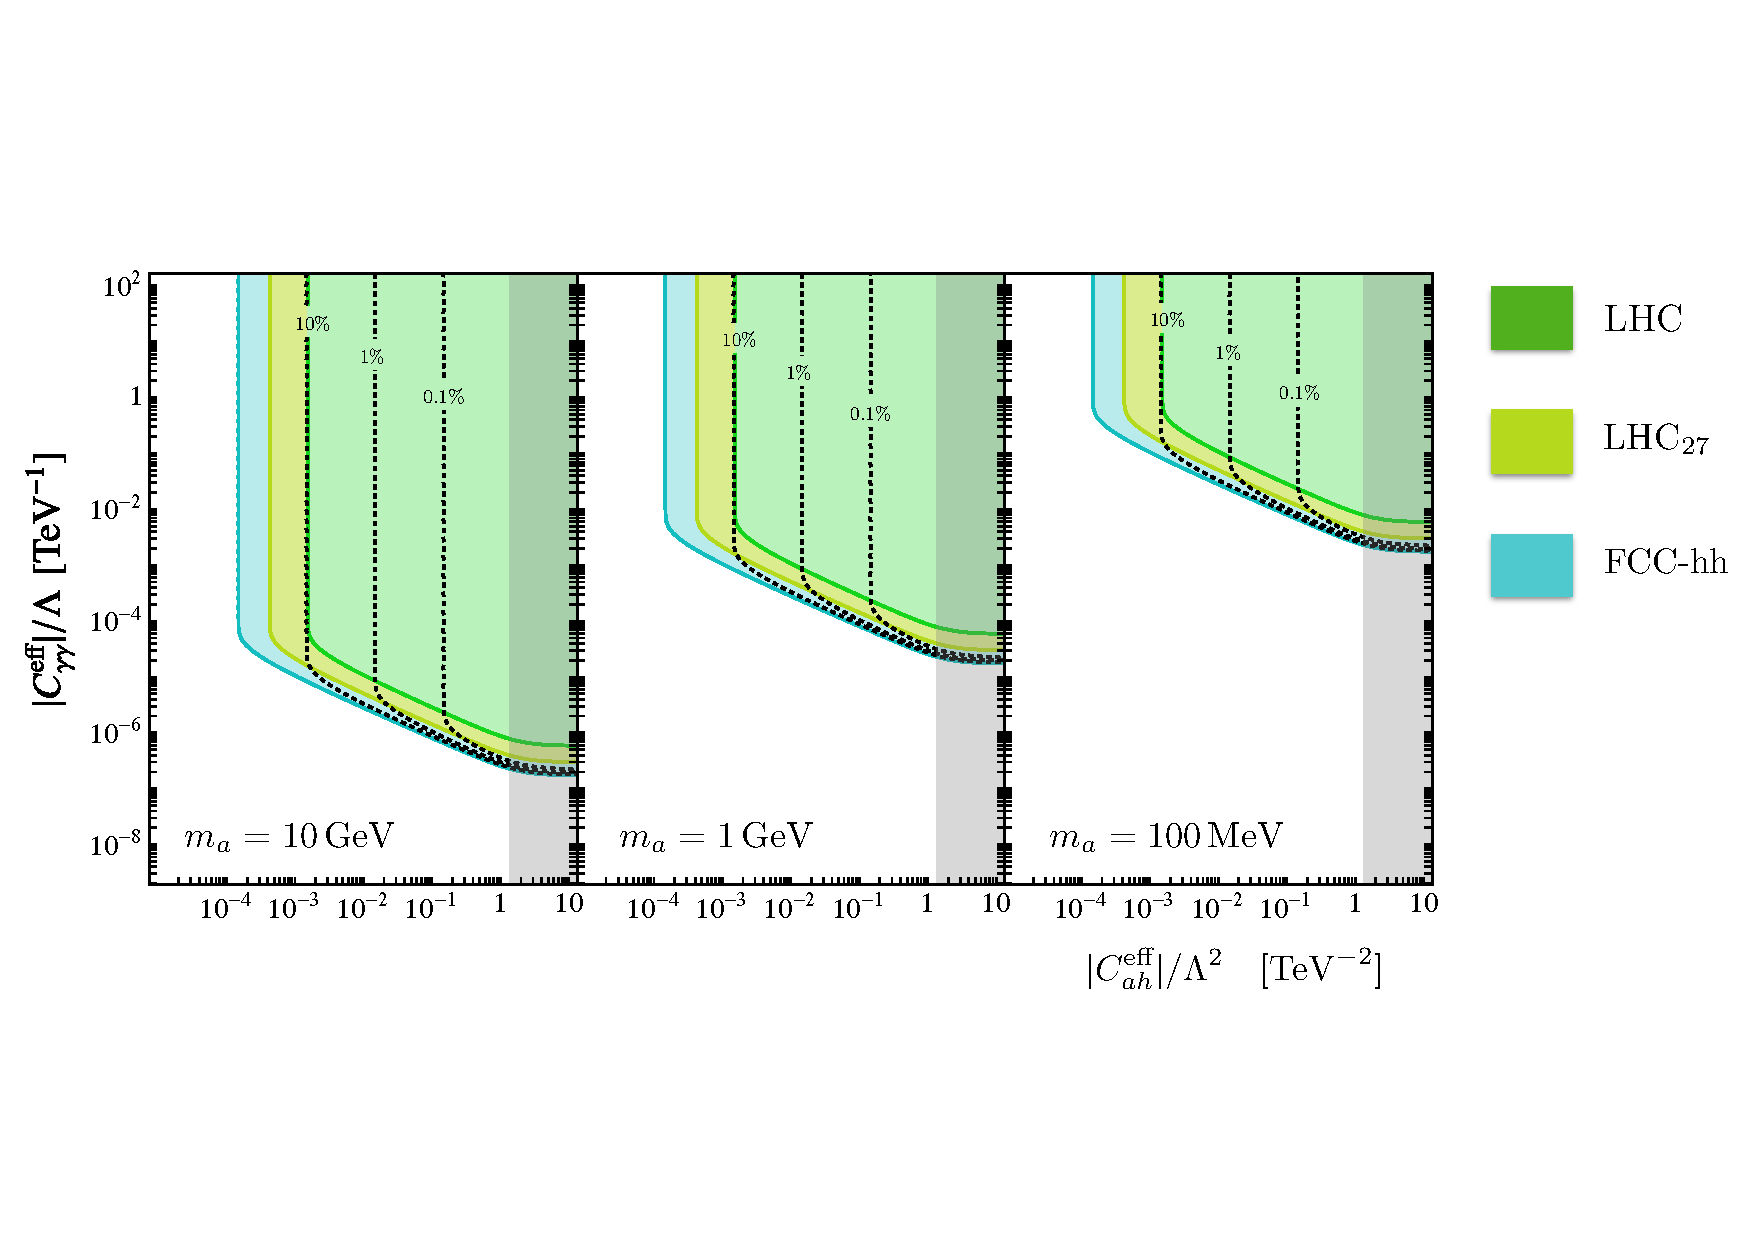
\includegraphics[width=0.85\textwidth]{\main/section9/plots/ALPs_hh_htoaa.pdf}
\end{center}
\vspace{-0mm}
\caption{\label{fig:pphZa} Projected reach in searches for $h \to Za \to \ell^+\ell^-+2\gamma $ and $h \to aa \to 4\gamma $ decays with the LHC with $3$\,ab$^{-1}$
(green), HE-LHC with $15$\,ab$^{-1}$ (light green) and a $100\,$TeV collider with $20$\,ab$^{-1}$ (blue). The parameter region with the solid contours correspond to a branching ratio of $\text{Br}(a\to 
\gamma\gamma)=1$, and the contours showing the reach for smaller branching ratios are dotted.}
\end{figure}
%%% ++++++++ 
%


Light or weakly coupled ALPs can be long-lived, and thus only a fraction of them decay inside the detector and can be reconstructed. The average ALP decay length perpendicular to the beam axis is given by
%
\begin{equation}\label{eq:Lperp}
   L_a^\perp(\theta) = \frac{\sqrt{\gamma_a^2 - 1}}{\Gamma_a}\,\sin\theta \,, 
\end{equation}
%
where $\Gamma_a$ denotes the total width of the ALP, $\theta$ is the scattering angle (in the center-of-mass frame) and $\gamma_a$ specifies the relativistic boost factor. Using the fact that most Higgs bosons are produced in the forward direction at the LHC and approximating the ATLAS and CMS detectors (as well as future detectors) by infinitely long cylindrical tubes, we first perform a Lorentz boost to the rest frame of the decaying boson. In this frame the relevant boost factors for the Higgs decay into ALPs are given by
 %
\begin{align}
\gamma_a=\begin{cases}\displaystyle{ \frac{m_h^2-m_Z^2+m_a^2}{2m_am_h}}\,,& \text{for}\,\, h \to Z a\,,\\[14pt]
\displaystyle \frac{m_h}{2m_a}\,,&\text{for}\,\, h \to aa\,.\\
\end{cases}
\end{align}
%
We can compute the fraction of ALPs decaying before they have travelled a certain distance $L_{\rm det}$ from the beam axis, finding 
%
\begin{equation}\label{eq:ffactors}
\begin{aligned}
   f_{\rm dec}^{a} &= \int_0^{\pi/2}\!d\theta \,  \sin\theta
    \left( 1 - e^{-L_{\rm det}/L_a^\perp(\theta)} \right) , \\
   f_{\rm dec}^{aa} &= \int_0^{\pi/2}\!d\theta \,  \sin\theta
    \left( 1 - e^{-L_{\rm det}/L_a^\perp(\theta)} \right)^2,
\end{aligned}
\end{equation} 
%
where $f^a_\text{dec}$ is relevant for $h \to Z a$ decays and $f^{aa}_\text{dec}$ applies to $h\to aa$ decays. 

For prompt ALP decays, we demand all final state particles to be detected in order to reconstruct the decaying SM particle. For the decay into photons we 
require the ALP to decay before the electromagnetic calorimeter which, at ATLAS and CMS, is situated approximately $1.5\,$m from the interaction point, and we thus take $L_{\rm det} = 
1.5\,$m. Analogously, the ALP should decay before the inner tracker, $L_{\rm det} = 2\,$cm, for an $e^+e^-$ final state to be detected. We also require $L_\text{det}
=2\,$cm for muon and tau final states in order to take full advantage of the tracker information in reconstructing these events. We define the effective branching ratios
%
\begin{align}
\text{Br}(h\to Za\to Y\bar{Y}+X\bar{X})\big\vert_\text{eff}&=\text{Br}(h\to Za)\,\text{Br}(a\to X\bar{X})f_\text{dec}^a\,\text{Br}(Z\to Y\bar{Y})\,,\label{eq:LHChZa}\\
\text{Br}(h\to aa\to X\bar{X}+X\bar{X})\big\vert_\text{eff}&=\text{Br}(h\to aa)\,\text{Br}(a\to X\bar{X})^2f_\text{dec}^{aa}\,,\label{eq:LHChaa}
\end{align}
%
where $X=\gamma, e, \mu, \tau$ and $Y=\ell, {\rm hadrons}$. Multiplying the effective branching ratios by the appropriate Higgs production cross section and luminosity allows us to derive results for a specific collider. The Higgs production cross section at $14\,$TeV is given by $\sigma(pp\to h)= 54.72\,$pb (see Sec.~\ref{sec2_HXSWG1} of this report). We use the reference cross section $\sigma(gg 
\to h) = 146.65\,$pb at $\sqrt{s} = 27\,$TeV. At $\sqrt{s} = 100\,$TeV, the relevant cross section is $\sigma(gg \to h) = 802\,$pb ~\cite{Mangano:2016jyj}. We require $100$ signal events, since this is what is typically needed to suppress backgrounds in new-physics searches with prompt Higgs decays \cite{Khachatryan:2016vau, Chatrchyan:2013vaa,Aad:2015bua} (see also \cite{Bauer:2017ris} for 
further discussion).
We do not take advantage of the additional background reduction obtained by cutting on a secondary vertex in the case where the ALP lifetime becomes appreciable. A dedicated analysis by the experimental collaborations including detailed simulations of the backgrounds is required to improve on our projections.  


%
%%% ++++++++ 
\begin{figure}[t]
\begin{center}
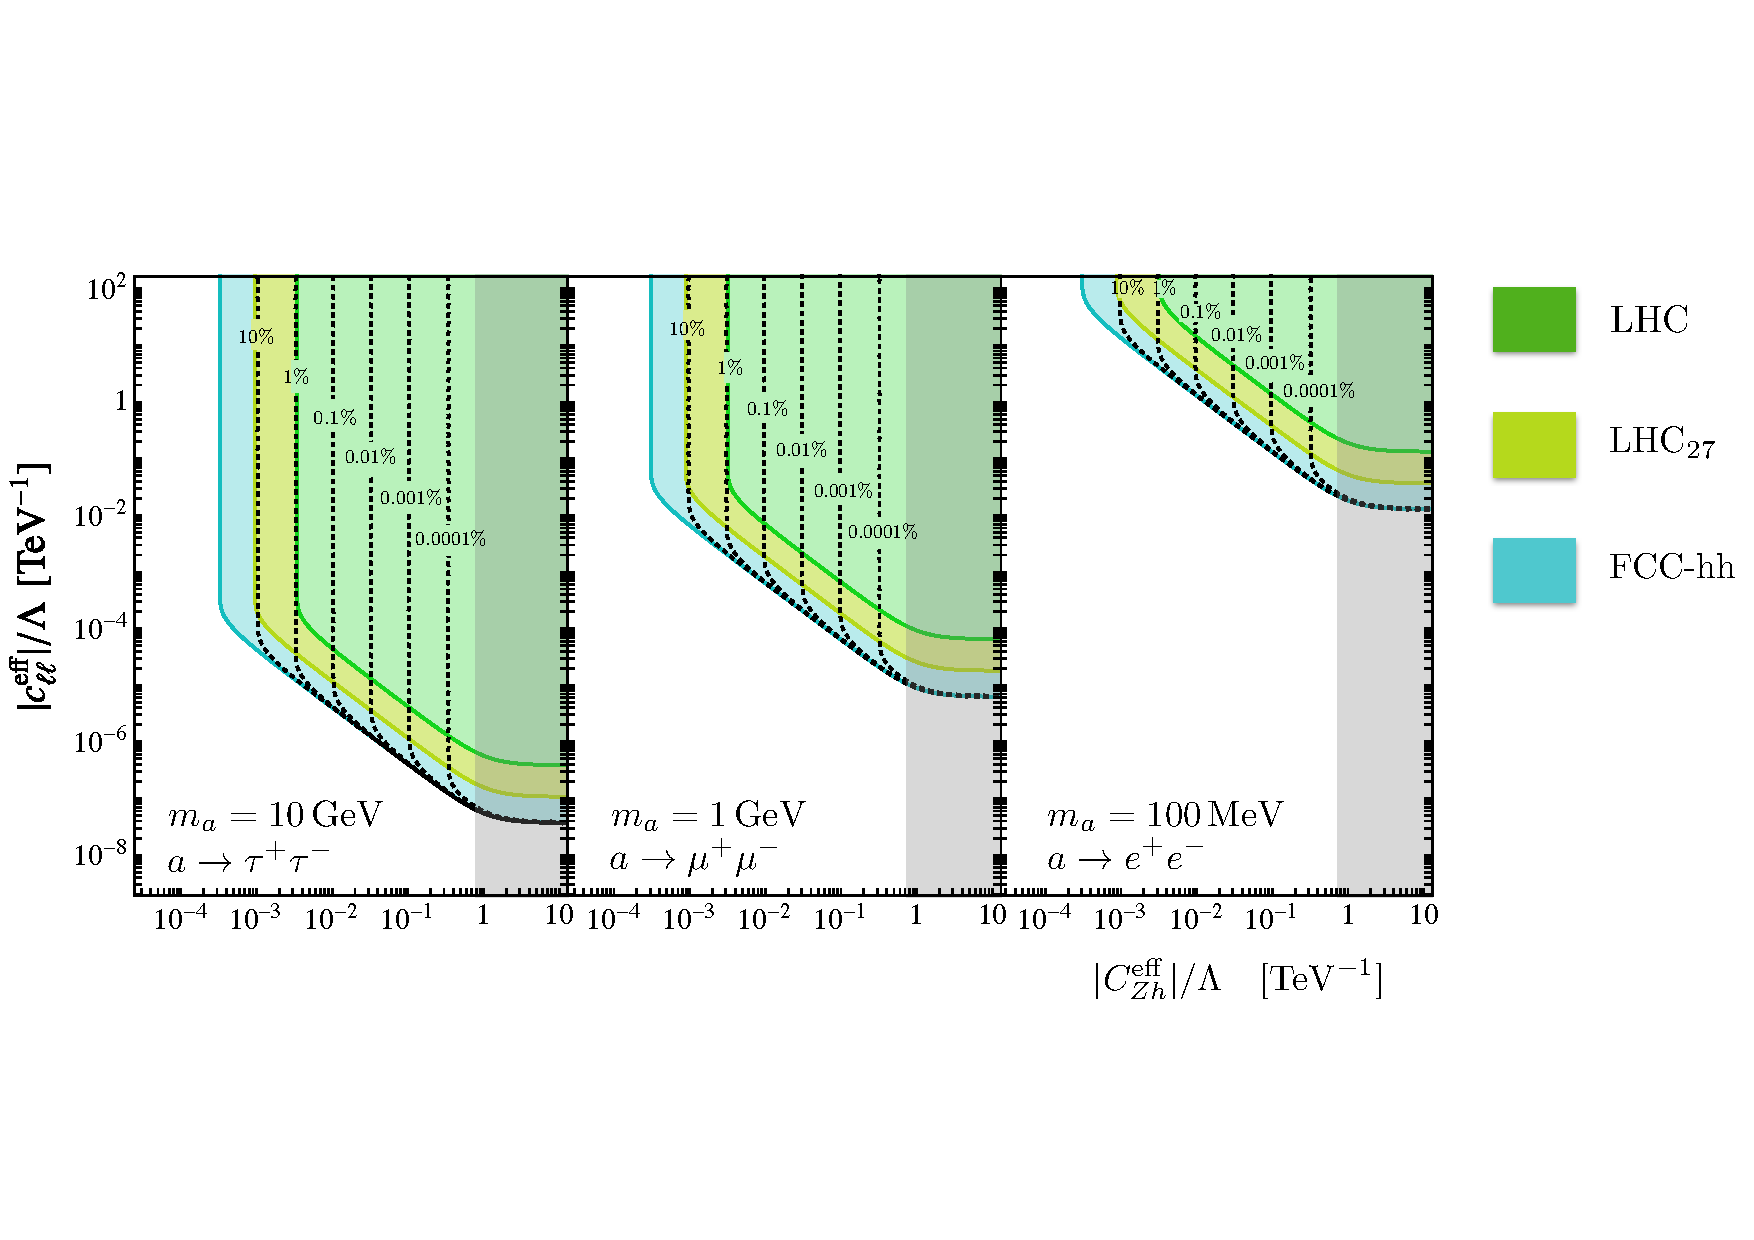
\includegraphics[width=0.85\textwidth]{\main/section9/plots/ALPs_hh_htoZa_lep.pdf}
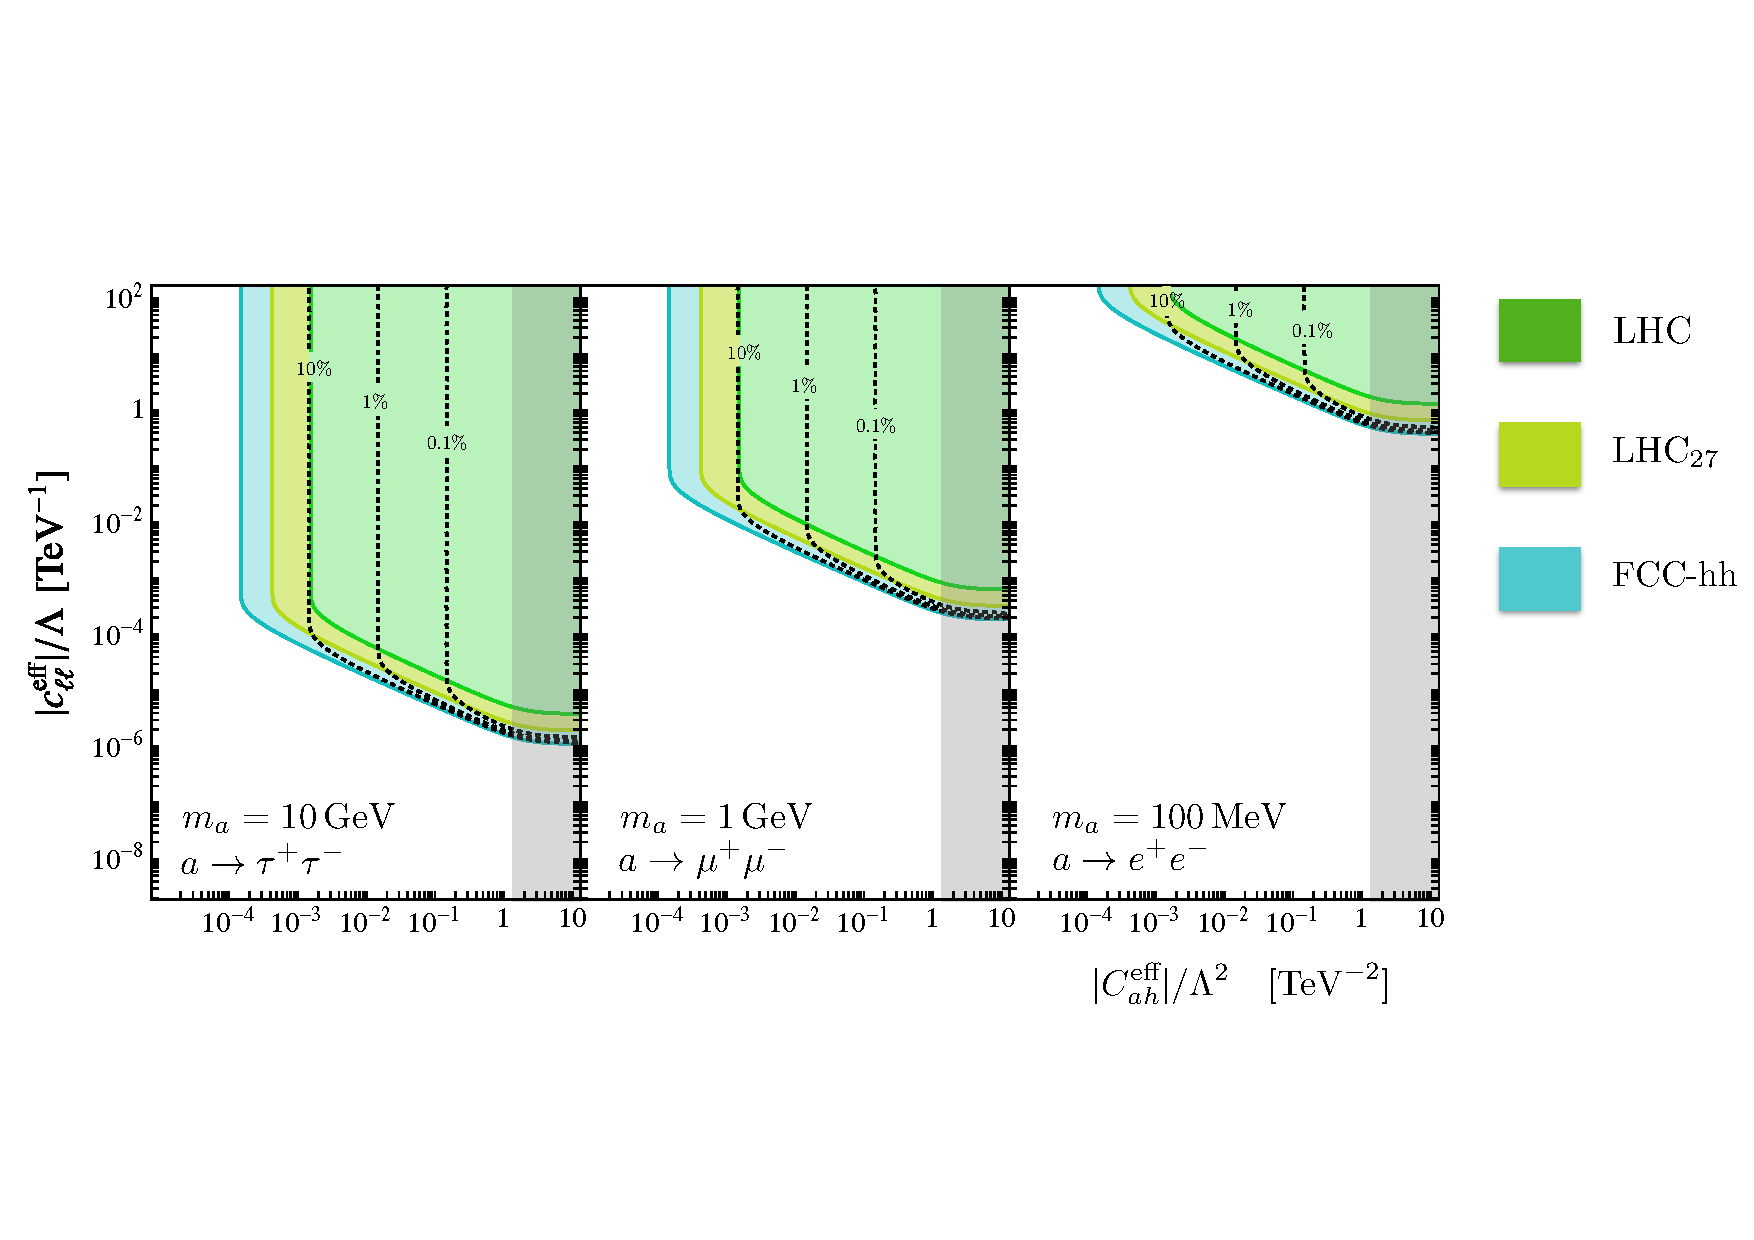
\includegraphics[width=0.85\textwidth]{\main/section9/plots/ALPs_hh_htoaa_lep.pdf}
\end{center}
\vspace{-3mm}
\caption{\label{fig:pphZalep} Projected reach in searches for $h \to Za \to \ell^+\ell^-+\ell^+\ell^- $ and $h \to aa \to 4\ell $ decays with the LHC with $3$\,ab$^{-1}$
(green), HE-LHC with $15$\,ab$^{-1}$ (light green) and a $100\,$TeV collider with $20$\,ab$^{-1}$ (blue). The parameter region with the solid contours correspond to a branching ratio of $\text{Br}(a\to 
\ell^+\ell^-)=1$, and the contours showing the reach for smaller branching ratios are dotted.}
\end{figure}
%%% ++++++++ 
%

In Figure~\ref{fig:pphZa}, we display the reach for observing 100 events at the HL-LHC, HE-LHC and FCC-hh (in green, light green and blue respectively) in searches for $pp\to h \to Za\to \ell^+\ell^-\gamma\gamma$ (upper panels) and  $pp\to h \to aa\to 4 \gamma$ (lower panels) for $m_a= 10\,$GeV, $1\,$GeV and $100\,$MeV (left, middle, right panel) in the $|C_{Zh}^{\rm eff}|/\Lambda - |C_{\gamma\gamma}^{\rm eff}|/\Lambda$ and $|C_{ah}^{\rm eff}|/\Lambda^2 - |C_{\gamma\gamma}^{\rm eff}|/\Lambda$ planes respectively. We assume $\text{Br}(a\to \gamma\gamma)=1$ and indicate the reach of the FCC-hh obtained in the case that $\text{Br}(a\to \gamma\gamma)<1$ by the black dotted lines. 
In $h \to Za$ searches, the HL-LHC can reach values of $|C_{Zh}^{\rm eff}|/\Lambda$ down to $3 \times 10^{-3} (\Lambda/\textrm{TeV})$ for all ALP masses. The HE-LHC improves this reach by a factor of $3$ to $1 \times 10^{-3} (\Lambda/\textrm{TeV})$, while the FCC-hh increases the reach by an order of magnitude to values as small as $3 \times 10^{-4} (\Lambda/\textrm{TeV})$. In $|C_{\gamma\gamma}^{\rm eff}|/\Lambda$, the HL-LHC is sensitive to values larger than $10^{-7}, 10^{-5}$ and $10^{-3} (\Lambda/\textrm{TeV})$ for $m_a = 10\,$GeV, $1\,$GeV and $100\,$MeV, respectively, and the largest allowed value of $|C_{Zh}^{\rm eff}|/\Lambda = 0.72\,(\Lambda/\textrm{TeV})$. The sensitivity of the HE-LHC (FCC-hh) increases by a factor $3$ ($10$). 

The process $h \to aa$ can access $|C_{ah}^{\rm eff}|/\Lambda^2 = 1.5, 0.4, 0.15 \times 10^{-3} (\Lambda/\textrm{TeV})^2$ at the HL-LHC, HE-LHC and FCC-hh, respectively. In $|C_{\gamma\gamma}^{\rm eff}|/\Lambda$, the HL-LHC is sensitive to values larger than $8 \times 10^{-7}, 8 \times 10^{-5}$ and $8 \times 10^{-3} (\Lambda/\textrm{TeV})$ for $m_a = 10\,$GeV, $1\,$GeV and $100\,$MeV, respectively, for the largest allowed value of $|C_{ah}^{\rm eff}|/\Lambda$. Both the HE-LHC as well as the FCC-hh improve this reach by a factor $2$ each. For all considered ALP masses, the $h\to Z a$ decay could be observed at a $100\,$TeV collider for $\text{Br}(a\to \gamma\gamma)\gtrsim 10^{-6}$ and the $h\to a a$ decay could be fully reconstructed for $\text{Br}(a\to \gamma\gamma)\gtrsim 0.01$.

The results are similar for leptonic ALP decays. In Figure~\ref{fig:pphZalep} we show the reach in the $|c_{\ell\ell}^\text{eff}|/\Lambda - |C_{Zh}^\text{eff}|/\Lambda$ plane (upper row) and  $|c_{\ell\ell}^\text{eff}|/\Lambda - |C_{ah}^\text{eff}|/\Lambda^2$ plane (lower row) for ALP decays into taus (left), muons (middle) and electrons (right). In $|C_{Zh}^\text{eff}|/\Lambda$ the reach coincides with the one of the same process with ALP decays into photons. For $h \to Za$ the HL-LHC can probe values $|c_{\ell\ell}^\text{eff}|/\Lambda = 6 \times 10^{-7}, 10^{-4}, 2 \times 10^{-1}\,(\Lambda/\textrm{TeV})$ for $m_a = 10\,$GeV, $1\,$GeV and $100\,$MeV, respectively. The HE-LHC (FCC-hh) increases this reach by a factor 3 (10). Similarly for $h \to aa$ the HL-LHC is sensitive to values $|c_{\ell\ell}^\text{eff}|/\Lambda = 6 \times 10^{-6}, 10^{-3}, 2 \,(\Lambda/\textrm{TeV})$ which the HE-LHC and FCC-hh can increase by a factor $2$ each.
